\documentclass[10pt]{beamer}
\usepackage[latin1]{inputenc}
\usepackage{amsmath}
\usepackage{amssymb}
\usepackage{graphics}
\usepackage{graphicx}
\usepackage{epsfig}
\usepackage{fancyhdr}
\usepackage{wasysym}
\usepackage{latexsym}
\usepackage{amsfonts}
\usepackage{subfigure}
\usepackage{color}
\usepackage[numbers]{natbib}
\usepackage{framed}
\usepackage{multirow}
\usepackage{booktabs}
\usepackage{chngpage}
\usepackage{caption}
\usepackage{tikz}
\usepackage{mdwlist}
\usepackage{algorithm,algorithmic,amsmath}



\DeclareMathOperator*{\argmax}{arg\,max}
\newcommand{\todo}[1]{\textcolor{red}{\textbf{TODO:} #1}}
\newcommand{\setD}{\ensuremath{D} }
\newcommand{\setW}{\ensuremath{V} }
\newcommand{\setC}{\ensuremath{C} }
\newcommand{\matD}{\ensuremath{\mathrm{D}} }
\newcommand{\matW}{\ensuremath{\mathrm{W}} }
\newcommand{\matC}{\ensuremath{\mathrm{C}} }
\newcommand{\vecdi}[1]{\ensuremath{\mathrm{v}^{D}_{#1}}}
\newcommand{\vecwi}[1]{\ensuremath{\mathrm{v}^{W}_{#1}}}
\newcommand{\vecci}[1]{\ensuremath{\mathrm{v}^{C}_{#1}}}
\newcommand{\con}{$(w_{t-c}, \ldots, w_{t-1}, w_{t+1}, \ldots, w_{t+c})$}
\newcommand{\wgt}[1]{\ensuremath{\lambda_{#1}}}
\newcommand{\traindata}{\ensuremath{\mathcal{T}}}
\newcommand{\db}{\ensuremath{\mathcal{D}} }
\newcommand{\para}[1]{\noindent\textbf{%\fontsize{14}{15}\selectfont 
#1}} %{\paragraph{#1}}
\newcommand{\highest}[1]{\textbf{#1}}

\usetheme{Madrid}
%\usetheme{umbc1}
\title[{Distributed Document Representations for Multi-Label Document Categorization}]{Learning Distributed Document Representations for Multi-Label Document Categorization}
\author{\textbf{Nitish Gupta}}
\date{May 16, 2015}
\institute[IITK]{B.Tech - M.Tech Dual Degree\\
\vspace{.2cm}Thesis Defense\\ 
\vspace{.2cm}Electrical Engineering\\
\vspace{.2cm}IIT Kanpur }
\begin{document}
\setbeamercovered{clear}
%%%%%%%%%%%%%%%%%%%%%%%%%%%% 
\begin{frame}
\titlepage
%\begin{figure}[ht]
%\begin{center}
%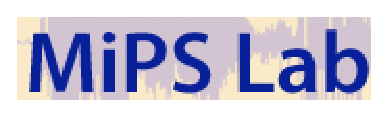
\includegraphics[width=1.75cm]{mips}
%\epsfig{file=iitk_logo.eps,width=1.5cm}
%\end{center}
%\end{figure}
\begin{figure}[ht]
\begin{center}
\includegraphics[width=1.75cm]{iitk_logo-eps-converted-to.pdf}
%\epsfig{file=iitk_logo.eps,width=1.5in}
\end{center}
\end{figure}
%\begin{figure}
%\begin{center}
%\hspace{-.0cm}
%\vspace{2cm}\includegraphics[width=1.25cm]{mips-eps-converted-to.pdf}
%\end{center}
%\end{figure}
\end{frame}

%%%%%%%%%%%%%%%%%%%%%%%%%%%%
\begin{frame}{Outline}
\begin{enumerate}
	\vfill\item Multi-Label Document Categorization
	\vfill\item Related Work
	\begin{itemize}
	  \vfill\item Text Representations
	  \vfill\item Learning Algorithms
	\end{itemize}  
	\vfill\item Distributed Word Representations
	\vfill\item Learning Distributed Document Represenations
	\vfill\item Document Cateogorization Algorithm
	\vfill\item Results
	\vfill\item Conclusion and Future Work
\end{enumerate}
\end{frame}

%%%%%%%%%%%%%%%%%%%%%%%%%%%%

\begin{frame}{Intoduction to Multi-Label Document Categorization}
\begin{itemize}
	\vfill\item<1-> Text Documents usually belong to more than one conceptual class. \\For E.g. an article on Music Piracy 
	\vfill\item<2-> Task of assigning documents to one or more predefined categories is called \emph{Multi-Label Document Categorization}
	\vfill\item<3-> Wide range real-world applications :
	\begin{itemize} 
	  \vfill\item<3-> Web-page tagging
	  \vfill\item<3-> Medical Patient Record Management
	  \vfill\item<3-> Wikipedia Article Management
	  \vfill\item<3-> Document Recommendation etc.
	\end{itemize} 
	\vfill\item<4-> Multi-label classification belongs to a general class of supervised learning algorithms where : 
	\begin{itemize}
	  \vfill\item<5-> Training instances in the form of document-category pairs are used to learn a classifier $\mathcal{H}$ 
	  \vfill\item<6-> Learned classifier $\mathcal{H}$ is used to assign categories to new test documents
	\end{itemize}
\end{itemize}
\vfill
\end{frame}

%%%%%%%%%%%%%%%%%%%%%%%%%%%%

\begin{frame}{Introduction to Multi-Label Document Categorization}
%\onslide<1->{ \textbf{Problem Statement}, } \\
\vfill\onslide<1->{ Given, }
\begin{itemize} 
	\vfill\item<1-> A set of documents $D = \{d_{1}, \ldots, d_{|D|}\}$
	\vfill\item<2-> A set of categories $C = \{c_{1}, \ldots, c_{|C|}\}$
	\vfill\item<3-> Training data for $n$ {\small ($n < |D|$)} documents, $\traindata = \{l_{d_{1}}, \ldots, l_{d_{n}}\}$ 
\onslide<4->{   \\ Each label vector $l_{d_{i}} \in \{0,1\}^{|C|}$ denotes relevance of categories to the document $d_{i}$ }
\end{itemize} 
\vfill
\onslide<5->{
	Example :
	\begin{table}[h!]
	\tabcolsep=0.1cm
	\tiny
	\begin{center}
	\begin{tabular}{c@{\hskip5mm} c c c c c c}
	\toprule
	\textbf{Documents}	&	\textbf{Sports} & \textbf{Music} & \textbf{Arts} & \textbf{Technology}  & \textbf{Literature} & \textbf{Politics}\\
	\cmidrule{1-1}
	\cmidrule{2-7}
	$d_{1}$ & 0 & 0 & 1 & 0 & 1 & 0\\
	$d_{2}$ & 0 & 1 & 1 & 0 & 0 & 1\\
	$d_{3}$ & 1 & 0 & 0 & 1 & 0 & 1\\
	$d_{4}$ & x & x & x & x & x & x\\
	$d_{5}$ & x & x & x & x & x & x\\
	\bottomrule         
	\end{tabular}
	\end{center}
	\end{table}
}
\vfill
\onslide<6->{
Using $\traindata$, $D$ and $C$ the learning algorithm learns a multi-label classifier $\mathcal{H}$ to estimate category label vectors, $l_{d_{j}}$ {\small $(j>n)$} for the test documents. 
}
\vfill
\end{frame}

%%%%%%%%%%%%%%%%%%%%%%%%%%%%

\begin{frame}{Introduction to Multi-Label Document Categorization}
\vfill\onslide<1->{ Document Categorization task has the following two components : }
\begin{enumerate}
	\vfill\item<2-> \emph{Learning Document Representations} : Representing text documents using numerical vectors that are inputs to the multi-label classifier $\mathcal{H}$
	\begin{itemize}
	 	\vfill\item<3-> Each document $d_{i} \in D$ is represented using a vector $v_{d_{i}} \in \mathbb{R}^{k}$ \\
	 	\vfill\item<4->	Vectors ($v_{d_{i}}$) should encode the semantic content of the documents 
	 	\vfill\item<5-> Encoding documents in a $k$-dimensional space using such represenation is called the \emph{Vector Space Model}
	 	\vfill\item<6-> The complete document set $D$ can be represented by a document representation matrix $\matD \in \mathbb{R}^{k \times |D|}$
	\end{itemize}
\suspend{enumerate} \vfill
\onslide<7->{	
\emph{ In this thesis, we focus on learning efficient document representations, $\matD$}	}
\vfill
	\resume{enumerate}
	\vfill\item<8-> \emph{Learning Algorithm} : Algorithm to learn the multi-label classifier $\mathcal{H}$
\end{enumerate}\vfill 
\end{frame}

%%%%%%%%%%%%%%%%%%%%%%%%%%%%

\begin{frame}{Background on Learning Algorithms}
\vfill
%\onslide<1->{ Learning algorithms can be classified into two classes :  }
\begin{enumerate}
	\vfill\item<2-> \emph{Learning Multiple Binary Classifiers} : \\
	\onslide<3->{ {\footnotesize	Algorithms that treat each category assignment independently and learn multiple binary classifiers, one for each category, to make the category assignments} 	} 
	\begin{itemize}
		\vfill\item<4-> Logistic Regression
		\vfill\item<5-> Support Vector Machines (SVM)
		\vfill\item<6-> Neural Networks
		\vfill\item<7-> Naive Bayes
	\end{itemize}

	\vfill\item<8-> \emph{Learning Single Joint Classifier} : \\
	\onslide<9->{ {\footnotesize	Algorithms that jointly assign all the categories to a document $d_{i}$, i.e. estimate the complete label vector $l_{d_{i}}$ using a single classifier} 	}
	\begin{itemize}
		\vfill\item<10-> k-Nearest Neighbor (k-NN)
		\vfill\item<11-> Linear Least Square Fit
		\vfill\item<12-> Decision Trees
		\vfill\item<13-> Generative Probabilistic Models
	\end{itemize}
\end{enumerate}
%\onslide<14->{ Learning a single joint classifier is usually better as it is able to exploit the category correlations }
\vfill
\end{frame}

%%%%%%%%%%%%%%%%%%%%%%%%%%%%%%

\begin{frame}{Background on Text Representation}
\vfill
\onslide<1->{
\textbf{Bag of Words Model} }
%Most common method to learn vector representations for a set of documents is the \emph{Bag of Words (BOW)} model 	}
\begin{itemize}
	\vfill\item<2-> Document $d_{i}$ represented by $v_{d_{i}} \in \mathbb{R}^{|V|}$
	\vfill\item<3-> Each element in $v_{d_{i}}$ denotes presence/absence of each word
	\vfill\item<4-> Weighing techniques employed to give importance to important terms
	\begin{itemize}
		\vfill\item<5-> Term Frequency (\emph{tf} )
		\vfill\item<5-> Inverse Document Frequency (\emph{idf} )
		\vfill\item<5-> Term Frequency - Inverse Document Frequency (\emph{tf-idf} ) : \emph{tf} $\times$\emph{idf}
	\end{itemize}
\end{itemize}
\vfill
\onslide<6->{
\textbf{Drawbacks of the Bag-of-Words model} }
\begin{itemize}
	\vfill\item<7-> High-dimensionality
	\vfill\item<8-> Sparsity
	\vfill\item<9-> Inability to encode word contexts
	\vfill\item<10-> Ignores word order
\end{itemize}
\vfill
% \todo{feature selection. Word Embeddings. Our document embedding. Our docu cate. Datasets. Results End}
% \vfill
\end{frame}

%%%%%%%%%%%%%%%%%%%%%%%%%%%%%%

\begin{frame}{Background on Feature Selection / Dimensionality Reduction}
\vfill
\onslide<1-> {
Techniques to deal with sparsity and high-dimensionality in BOW }
\begin{itemize}
	\vfill\item<2-> Information Gain \\
	\onslide<2->{ { \scriptsize
	\begin{equation}
	G(t) = -\sum_{i=1}^{|C|} P(c_{i})\log P(c_{i}) + P(t)\sum_{i=1}^{|C|} P(c_{i}|t)\log P(c_{i}|t) + P(\sim t)\sum_{i=1}^{|C|} P(c_{i}|\sim t)\log P(c_{i}|\sim t)
	\end{equation}
	} }
	\vfill\item<3-> Mutual Information \\
	\onslide<3->{ { \scriptsize
	\begin{equation}
	I(t,c) = \log \frac{P(t \wedge c)}{P(t) \times P(c)} \text{,}\qquad I_{avg}(t) = \sum_{i=1}^{|C|} P(c_{i})I(t,c_{i})
	\end{equation}
	} }
	\vfill\item<4-> Latent Semantic Indexing (LSI) \\
	\onslide<4->{ { \scriptsize
	\begin{equation}
	X = T S D^{T}
	\end{equation}
	} }
\end{itemize}
\vfill
\end{frame}

% %%%%%%%%%%%%%%%%%%%%%%%%%%%%%%

\begin{frame}{Distributed Word Representations}
%\vfill
\onslide<1->{
Representating each word $w_{i}$ using vector $v_{w_{i}} \in \mathbb{R}^{k}$ ($k \in [50, 300]$) } \\ \vspace{0.5cm}
\onslide<2->{
\textbf{ Need for Distributed Word Representations} } 
\begin{itemize}
	\vfill\item<3-> Curse of Dimensionality
	\begin{itemize}
		\vfill\item<4-> One-hot representations grow with the size of vocabulary
		\vfill\item<5-> Parameters in language modelling grow exponentially with the size of vocabulary
	\end{itemize}
	\vfill\item<6-> No Word Similarity Measure
	\begin{itemize}
		\vfill\item<7-> One-hot representations are orthogonal representations
		\vfill\item<8-> Cannot capture semantic similarity between words
	\end{itemize}
\end{itemize}
\vfill
\end{frame}

%%%%%%%%%%%%%%%%%%%%%%%%%%%%%%
\begin{frame}{Neural Probabilistic Language Model}
\vfill
\onslide<1->{
\citet{bengio2003neural} developed \emph{Neural Probabilistic Language Model (NPLM)} to learn}%learn distributed word vectors and a probability function that uses these vectors to learn a statistical model of language	}
\begin{enumerate}
\vfill\item<2-> Distributed word vectors
\vfill\item<3-> A probability function that, using these word vectors, learns a statistical model of language 
\end{enumerate}

\begin{columns}[T]
 \begin{column}{.5\textwidth}
 	\centering
 	\onslide<4->{
 	\includegraphics[scale=0.15]{../figs/bengio_nn.png} }

 \end{column}

 \begin{column}{.5\textwidth}
 	\centering
 	{\footnotesize
 	\vfill \onslide<5->{
 	\begin{equation}
    P(w_{t} | w_{1}^{t-1}) \approx P(w_{t} | w_{t-n+1}^{t-1})
    \end{equation} }
    \vfill \onslide<6->{
    \begin{equation}
	y = b + U tanh(d + Hx) \text{,} \quad y \in \mathbb{R}^{|V|}
	\end{equation} }
	\vfill \onslide<7->{
	\begin{equation}
	P(w_{t} = i | w_{t-1}, \ldots, w_{t-n+1}) = \frac{e^{y_{w_t}}}{\sum_{i}e^{y_{i}}}
	\end{equation} }
	}
 \end{column}
\end{columns}

\vfill
\end{frame}

%%%%%%%%%%%%%%%%%%%%%%%%%%%%%%

\begin{frame}{Log-Linear Models}
\vfill
\onslide<1->{
\emph{Log-Linear Models} for learning distributed word vectors are proposed in \citet{mikolov2013efficient}. These models use word vectors to predict other words in the context.	 }
% \begin{itemize}
% \vfill\item<2-> do not build a language model hence also consider future words in contexts
% \vfill\item<3-> show that the word vectors capture the semantic similarity between words
% \end{itemize}
\vfill
\begin{enumerate}
	\vfill\item<2-> Continuous Bag-of-Words Model 
	\begin{columns}[T]

	 \begin{column}{.5\textwidth}
	 	\centering
	 	\onslide<2->{
	 	\includegraphics[scale=0.12]{../figs/mikolov_cbow.png} }
	 \end{column}
	 \begin{column}{.5\textwidth}
	 	\centering
	 	{\footnotesize
	 	\onslide<3->{
	 	\begin{equation}
	    h = w_{t-k} + \ldots + w_{t-1} + w_{t+1} + \dots + w_{t+k}
	    \end{equation} }
	    \onslide<4->{
	    \begin{equation}
		y = b + Uh \text{,} \quad y \in \mathbb{R}^{|V|}
		\end{equation} }
		\onslide<5->{
		\begin{equation}
		P(w_{t}|w_{t-k}, \ldots, w_{t+k}) = \frac{e^{y_{w_t}}}{\sum_{i} e^{y_{i}}}
		\end{equation} }
		}
	 \end{column}
	\end{columns}

	\vfill\item<6-> Skip-Gram Model
	\begin{columns}[T]

	 \begin{column}{.5\textwidth}
	 	\centering
	 	\onslide<6->{
	 	\includegraphics[scale=0.12]{../figs/mikolov_skip.png} }
	 \end{column}
	 \begin{column}{.5\textwidth}
	 	\centering
	 	\vfill
	 	{\footnotesize
	 	\onslide<7->{
	 	\begin{equation}
	    P(w_{t+j}|w_{t}) = \frac{e^{(v_{w_{t}} \cdot v_{w_{t+j}} )} }{\sum_{i} e^{(v_{w_{t}} \cdot v_{w_{i}})} }
	    \end{equation} }
	    }
	 \end{column}
	\end{columns}
\end{enumerate}

\vfill
\end{frame}

%%%%%%%%%%%%%%%%%%%

\begin{frame}{Distributed Document Representations}
\vfill \onslide<1->{
\textbf{Motivation for learning distributed document representations} }
\begin{enumerate}
	\vfill\item<2-> Traditional representations do not encode semantic similarity between documents. Therefore, cannot handle synonyms
	\vfill\item<3-> Drawbacks in BOW like sparsity, high-dimensionality, inability to encode context information and consider word ordering
	\vfill\item<4-> Compositionality of word vectors beyond weighted average \cite{mitchell2010composition, zanzotto2010estimating, yessenalina2011compositional, grefenstette2013multi, mikolov2013distributed} is not simple
	\vfill\item<5-> \citet{socher2013recursive} propose a Recursive Tensor Neural Network (RTNN) to compose word vectors for learning sentence representations using the parse-tree of the sentence in a bottom-up fashion
	\begin{itemize}
		\vfill\item<6-> Parsing, a computationally expensive step required for each sentence
		\vfill\item<7-> Composing sentence vectors to represent documents is not straight-forward
	\end{itemize}
\end{enumerate}
\end{frame}

% %%%%%%%%%%%%%%%%%%%%%%%%%%%%%%%%%%%%%%%%%%


\begin{frame}{Our Model for Learning Document Representations}
\vfill \onslide<1->{
\emph{Inspired by the log-linear models to learn word vectors, we present model, to learn universal distributed representations for documents and words } 
% \begin{quote}
% To learn universal distributed representations for documents and words
% \end{quote}
}
\vfill \onslide<2->{
\textbf{Hypothesis } 
\begin{quote}
Document Representations that encode semantic content of the document should be able to predict words in the document
\end{quote}}

\vfill \onslide<3->{
Our model, }
\begin{enumerate}
	\vfill\item<4-> Learns distributed representations for document (and words) that encode the different semantic content in the documents
	\vfill\item<5-> Embeds documents and words in the same $k$-dimensional space such that semantically similar entities have similar vector representations
\end{enumerate}

\end{frame}
% %%%%%%%%%%%%%%%%%%%%%%%%%%%%%%%%%%%%%%%%%%

\begin{frame}{Our Model for Learning Document Representations}
% \vfill\onslide<1->{
% We present an unsupervised neural network model that, }
% \begin{enumerate}
% 	\vfill\item<1-> Represents each document and word with a $k$-dimensional vector
% 	\vfill\item<2-> Estimates the probability of predicting the middle word in a given word sequence
% 	\vfill\item<3-> Learns document and word vectors and the parameters of the probability function using training corpus
% \end{enumerate}	
\vfill\onslide<1->{
We present an unsupervised neural network model that, }
\begin{enumerate}
	\vfill\item<2-> Represents each document $d_{i} \in D$ by a vector $\vecdi{i} \in \mathbb{R}^{k}$\\
	Vectors are stored as columns of the matrix $\matD = \left[\vecdi{1}, \ldots, \vecdi{|\setD|}\right] \in \mathbb{R}^{k \times |\setD|}$
	\vfill\item<3-> Each word $w_{i} \in W$, is represented by a vector $\vecwi{i} \in \mathbb{R}^{k}$
	Vectors are stored as columns of the matrix $\matW = \left[\vecwi{1}, \ldots, \vecwi{|\setW|}\right] \in \mathbb{R}^{k \times |\setW|}$
	\vfill\item<4-> Given a sequence of words, $(w_{t-c}, \ldots, w_{t+c})$ in document $d_{i}$, estimates 
	\begin{equation*}
	p(w_{t} | d_{i}, w_{t-c}, \ldots, w_{t-1}, w_{t+1}, \ldots, w_{t+c})
	\end{equation*}
	\vfill\item<5-> Maximizes the probability of predicting the words correctly to learn $\matD$ and $\matW$ and the parameters of the probability function
\end{enumerate}	
\end{frame}

% %%%%%%%%%%%%%%%%%%%%%%%%%%%%%%%%%%%%%%%%%%

\begin{frame}{Our Model for Learning Document Representations}
\vfill
\begingroup
\centering
\tikzset{every picture/.style={scale=0.4}}
\usetikzlibrary{calc}

\def\layersep{3.5cm}

\begin{tikzpicture}[shorten >=1pt,->,draw=black!50, node distance=\layersep,transform shape,rotate=90]  %<-- rotate the NN
	
	\newcommand{\inputsep}{2}
	\newcommand{\docnodey}{0}
	\newcommand{\docinputsep}{2.0}
	\newcommand{\docmiddlesep}{3.2}
	\newcommand{\wordneuron}{1.2}
	

	\newcommand{\iy}{\docnodey - \docinputsep}
	\newcommand{\iiy}{\docnodey - \docinputsep - \inputsep}
	\newcommand{\iiiy}{\docnodey - \docinputsep - \inputsep - \inputsep}
	\newcommand{\iiiiy}{\docnodey - \docinputsep - \inputsep - \inputsep - \inputsep}
	\newcommand{\mwy}{\docnodey + \docmiddlesep}
	\newcommand{\edgestyle}{below}

	\newcommand{\word}[1]{\parbox[t][][r]{8mm}{\centering \footnotesize #1}}

    \tikzstyle{every pin edge}=[<-,shorten <=1pt]
    \tikzstyle{neuronrect}=[rectangle,fill=black!25, minimum size=17pt, inner sep=0pt] %
    \tikzstyle{neuroncircle}=[circle,fill=black!25,minimum size=17pt,inner sep=0pt]
    \tikzstyle{vecrect} = [draw,fill=green!50, minimum width=0.2,minimum height=1cm]
    \tikzstyle{docrect} = [draw,fill=purple!50, minimum width=0.2,minimum height=1cm]
    \tikzstyle{hrect} = [draw,fill=blue!50, minimum width=0.2,minimum height=1cm]
    \tikzstyle{input neuron}=[neuronrect, fill=green!50];
    \tikzstyle{doc neuron}=[neuronrect, fill=purple!50];
    \tikzstyle{output neuron}=[neuroncircle, fill=red!50];
    \tikzstyle{hidden neuron}=[neuronrect, fill=blue!50];
    \tikzstyle{annot} = [text width=4em, text centered]
    \tikzset{hoz/.style={rotate=-90}}   %<--- for labels
    % Draw the input layer nodes
    %\foreach \name / \y in {1,...,4}
    % This is the same as writing \foreach \name / \y in {1/1,2/2,3/3,4/4}
        %\node[input neuron, pin=left:\rotatebox{-90}{\parbox[t][][r]{8mm}{\centering $w_{t-j}$}}] (I-\name) at (0,-\y) {};

    %Centre Word    
    \node[pin=left:\rotatebox{-90}{\word{Metallica}}] (I-1) at (-\wordneuron,\mwy) {};
	%\node[input neuron, pin=left:\rotatebox{-90}{\parbox[t][][r]{8mm}{\centering $w_{t}$}}] (W-0) at (0,\mwy) {};    
	\node[vecrect, pin=left:\rotatebox{-90}{\parbox[t][][r]{8mm}{\centering $w_{t}$}}] (W-0) at (0,\mwy) {};    

	%\node (rect) at (4,2) [draw,thick,fill=green!50, minimum width=0.2,minimum height=2cm, pin=left:\rotatebox{-90}{\word{Rolling\\Stones}}] {};
	
	%Doc 
	\node[pin=left:\rotatebox{-90}{\word{Rolling\newline Stones}}] (I-1) at (-\wordneuron,\docnodey) {};
    %\node[doc neuron, pin=left:\rotatebox{-90}{\parbox[t][][r]{8mm}{\centering $d_{i}$}}] (D-0) at (0,\docnodey) {};    
    \node[docrect, pin=left:\rotatebox{-90}{\parbox[t][][r]{8mm}{\centering $d_{i}$}}] (D-0) at (0,\docnodey) {};    

    \node[pin=left:\rotatebox{-90}{\word{metal}}] (I-1) at (-\wordneuron,\iy) {};
    %\node[input neuron, pin=left:\rotatebox{-90}{\parbox[t][][r]{8mm}{\centering $w_{t-2}$}}] (W-1) at (0,\iy) {};
    \node[vecrect, pin=left:\rotatebox{-90}{\parbox[t][][r]{8mm}{\centering $w_{t-2}$}}] (W-1) at (0,\iy) {};

    \node[pin=left:\rotatebox{-90}{\word{band}}] (I-1) at (-\wordneuron,\iiy) {};
    %\node[input neuron, pin=left:\rotatebox{-90}{\parbox[t][][r]{8mm}{\centering $w_{t-1}$}}] (W-2) at (0,\iiy) {};
    \node[vecrect, pin=left:\rotatebox{-90}{\parbox[t][][r]{8mm}{\centering $w_{t-1}$}}] (W-2) at (0,\iiy) {};
    
    \node[pin=left:\rotatebox{-90}{\word{plays}}] (I-1) at (-\wordneuron,\iiiy) {};
    %\node[input neuron, pin=left:\rotatebox{-90}{\parbox[t][][r]{8mm}{\centering $w_{t+1}$}}] (W-3) at (0,\iiiy) {};
    \node[vecrect, pin=left:\rotatebox{-90}{\parbox[t][][r]{8mm}{\centering $w_{t+1}$}}] (W-3) at (0,\iiiy) {};

    \node[pin=left:\rotatebox{-90}{\word{today}}] (I-1) at (-\wordneuron,\iiiiy) {};
    \node[vecrect, pin=left:\rotatebox{-90}{\parbox[t][][r]{8mm}{\centering $w_{t+2}$}}] (W-4) at (0,\iiiiy) {};    
    %\node[input neuron, pin=left:\rotatebox{-90}{\parbox[t][][r]{8mm}{\centering $w_{t+2}$}}] (W-4) at (0,\iiiiy) {};    

    % Draw the hidden layer nodes
    % \foreach \name / \y in {1,...,5}
        \path[yshift=0.5cm]
        %node[hidden neuron] (P-1) at (\layersep,\iy - 1) [label=below:\rotatebox{-90}{\parbox[t][][r]{2mm}{\centering \footnotesize $h_{c}$}}] {};
        node[hrect] (P-1) at (\layersep,\iy - 1) [label=below:\rotatebox{-90}{\parbox[t][][r]{2mm}{\centering \footnotesize $h_{c}$}}] {};

    % Draw the output layer node
    \node[output neuron, pin={[pin edge={->}]right:\rotatebox{-90}{$p(w_{t}|d_{i}, w_{t-2}, w_{t-1}, w_{t+1}, w_{t+2})$}}] (O) at (\layersep + \layersep,0) {};
    %\node[output neuron,pin={[pin edge={->}]right:\rotatebox{-90}{$p(w_{t}|d_{i}, w_{t-2}, \ldots, w_{t+2})$}}, right of=H-1] (O) {};

    % Connect word vectors to projection later
     \path (W-1) edge node[\edgestyle] {\rotatebox{-90}{\tiny $\wgt{t-2}$}} (P-1);
     \path (W-2) edge node[\edgestyle] {\rotatebox{-90}{\tiny $\wgt{t-1}$}} (P-1);
     \path (W-3) edge node[\edgestyle] {\rotatebox{-90}{\tiny $\wgt{t+1}$}} (P-1);
     \path (W-4) edge node[\edgestyle] {\rotatebox{-90}{\tiny $\wgt{t+2}$}} (P-1);   

    %Connect Middle Word to Output Node
	\path [->,font=\scriptsize] (W-0) edge (O);            

	%Connect Doc Embedding to Projection Layer
	\path (D-0) edge (P-1);            

    %Connect Projection Layer to Output
    \path (P-1) edge (O);

    % Annotate the layers
    \node[annot,above of=P-1, node distance=7.1cm,hoz] (hl) {\footnotesize Projection layer};
    \node[annot,left of=hl,hoz] {\footnotesize Input layer};
    \node[annot,right of=hl,hoz] {\footnotesize Output layer};
\end{tikzpicture}

% \begin{tikzpicture}[scale=1.0, transform shape]
% % Macros
% % relative positioning
% \newcommand{\at}[3]{
%   \begin{scope}[shift={(#1,#2)}]
%     #3
%   \end{scope} 
% }

% % Embeddings
% \newcommand{\embcolor}{PineGreen}
% \newcommand{\ye}{1}
% \newcommand{\he}{1.5}
% \newcommand{\we}{1}
% \newcommand{\gape}{1}

% \newcommand{\xc}{0.5}
% \newcommand{\xa}{\xc+\we+\gape}
% \newcommand{\xb}{\xa+\we+\gape}
% \newcommand{\xu}{\xb+\we+\gape}
% \newcommand{\xw}{\xu+\we+\gape}

% \draw [thick]
% 	(\xb+\we/2,\ye+\he+0.5) node[above,\embcolor] {Entities, $\mathcal{E}$};
% % Draw curly braces using path decoration
% \draw [\embcolor,decorate,decoration={brace,amplitude=5pt},xshift=-15pt] %,yshift=-9pt] 
% 	(\xc,\ye)  -- (\xc,\ye+\he) node [align=right,left,\embcolor,midway,xshift=-5pt]
% 	{Model Parameters, $\Phi$\\{\small $k$-dimensional entity vectors}};
% % Users
% \draw[<->,\embcolor!50]
% 	(\xu,\ye-0.15) -- (\xu+\we,\ye-0.15) 
% 	node[pos=.5,shape=rectangle,fill=white,draw=none] {\scriptsize $k$};
% \draw[<->,\embcolor!50] 
% 	(\xu+\we+0.3,\ye) -- (\xu+\we+0.3,\ye+\he) 
% 	node[pos=.5,shape=rectangle,fill=white,draw=none] {\scriptsize $|U|$};
% \draw [semithick,fill=gray!10] 
% 	(\xu,\ye) rectangle (\xu+\we,\ye+\he)
% 	(\xu+\we/2.0,\ye+\he/2.0) node[draw=none,shape=circle] (nodeU) {$\Phi_U$}
% 	(\xu+\we/2.0,\ye+\he) node[above] {\scriptsize Users, U};
% % Businesses
% \draw[<->,\embcolor!50]
% 	(\xb,\ye-0.15) -- (\xb+\we,\ye-0.15) 
% 	node[pos=.5,shape=rectangle,fill=white,draw=none] {\scriptsize $k$};
% \draw[<->,\embcolor!50] 
% 	(\xb+\we+0.3,\ye) -- (\xb+\we+0.3,\ye+\he) 
% 	node[pos=.5,shape=rectangle,fill=white,draw=none] {\scriptsize $|B|$};
% \draw [semithick,fill=gray!10] 
% 	(\xb,\ye) rectangle (\xb+\we,\ye+\he)
% 	(\xb+\we/2.0,\ye+\he/2.0) node[draw=none,shape=circle] (nodeB) {$\Phi_B$}
% 	(\xb+\we/2.0,\ye+\he) node[above] {\scriptsize Businesses, B};
% % Categories
% \draw[<->,\embcolor!50]
% 	(\xc,\ye-0.15) -- (\xc+\we,\ye-0.15) 
% 	node[pos=.5,shape=rectangle,fill=white,draw=none] {\scriptsize $k$};
% \draw[<->,\embcolor!50] 
% 	(\xc+\we+0.3,\ye) -- (\xc+\we+0.3,\ye+\he) 
% 	node[pos=.5,shape=rectangle,fill=white,draw=none] {\scriptsize $|C|$};
% \draw [semithick,fill=gray!10] 
% 	(\xc,\ye) rectangle (\xc+\we,\ye+\he)
% 	(\xc+\we/2.0,\ye+\he/2.0) node[draw=none,shape=circle] (nodeC) {$\Phi_C$}
% 	(\xc+\we/2.0,\ye+\he) node[above] {\scriptsize Categories, C};
% % Attributes
% \draw[<->,\embcolor!50]
% 	(\xa,\ye-0.15) -- (\xa+\we,\ye-0.15) 
% 	node[pos=.5,shape=rectangle,fill=white,draw=none] {\scriptsize $k$};
% \draw[<->,\embcolor!50] 
% 	(\xa+\we+0.3,\ye) -- (\xa+\we+0.3,\ye+\he) 
% 	node[pos=.5,shape=rectangle,fill=white,draw=none] {\scriptsize $|A|$};
% \draw [semithick,fill=gray!10] 
% 	(\xa,\ye) rectangle (\xa+\we,\ye+\he)
% 	(\xa+\we/2.0,\ye+\he/2.0) node[draw=none,shape=circle] (nodeA) {$\Phi_A$}
% 	(\xa+\we/2.0,\ye+\he) node[above] {\scriptsize Attributes, A};
% % Words
% \draw[<->,\embcolor!50]
% 	(\xw,\ye-0.15) -- (\xw+\we,\ye-0.15) 
% 	node[pos=.5,shape=rectangle,fill=white,draw=none] {\scriptsize $k$};
% \draw[<->,\embcolor!50] 
% 	(\xw+\we+0.3,\ye) -- (\xw+\we+0.3,\ye+\he) 
% 	node[pos=.5,shape=rectangle,fill=white,draw=none] {\scriptsize $|W|$};
% \draw [semithick,fill=gray!10] 
% 	(\xw,\ye) rectangle (\xw+\we,\ye+\he)
% 	(\xw+\we/2.0,\ye+\he/2.0) node[draw=none,shape=circle] (nodeW) {$\Phi_W$}
% 	(\xw+\we/2.0,\ye+\he) node[above] {\scriptsize Review words, W};

% % Matrices (Relations)
% \newcommand{\relcolor}{RoyalBlue}
% \newcommand{\ym}{-2}
% \newcommand{\hm}{2}
% \newcommand{\wm}{2}
% \newcommand{\gapm}{0.75}
% \newcommand{\gridmcolor}{gray!10}

% \newcommand{\xCB}{-2}
% \newcommand{\xAB}{\xCB+\wm+\gapm}
% \newcommand{\xR}{\xAB+\wm+\gapm}
% \newcommand{\xBW}{\xR+\wm+\gapm}
% \newcommand{\xUW}{\xBW+\wm+\gapm}

% \newcommand{\sparsegrid}{
% 	\draw [step=0.1,thin,\gridmcolor] (0,0) grid (\wm,\hm);
% 	\foreach \i in {0,1,...,75}{
% 		\pgfmathsetmacro{\xcell}{int(rnd*20)*\wm/20}
% 		\pgfmathsetmacro{\ycell}{int(rnd*20)*\wm/20}
% 		\fill[gray!20] (\xcell,\ycell) rectangle (\xcell+0.1,\ycell+0.1);
% 	}
% }

% \draw [thick]
% 	(\xR+\wm/2,\ym-0.5) node[below,\relcolor] {Relations, $\mathcal{R}$};
% % Draw curly braces using path decoration
% \draw [\relcolor,decorate,decoration={brace,amplitude=5pt},xshift=-15pt] %,yshift=-9pt] 
% 	(\xCB,\ym)  -- (\xCB,\ym+\hm) node [align=right,left,\relcolor,midway,xshift=-5pt]
% 	{Partial Observations\\{\small Predict missing data}};

% % CB
% \draw[<->,\relcolor!50]
% 	(\xCB,\ym+\hm+0.15) -- (\xCB+\wm,\ym+\hm+0.15) 
% 	node[pos=.5,shape=rectangle,fill=white,draw=none] {\scriptsize $|C|$};
% \draw[<->,\relcolor!50] 
% 	(\xCB+\wm+0.3,\ym) -- (\xCB+\wm+0.3,\ym+\hm) 
% 	node[pos=.5,shape=rectangle,fill=white,draw=none] {\scriptsize $|B|$};
% \at{\xCB}{\ym}{\sparsegrid}
% \draw [thick] 
% 	(\xCB,\ym) rectangle (\xCB+\wm,\ym+\hm)
% 	(\xCB+\wm/2.0,\ym+\hm/2.0) node[draw=none,shape=circle] (nodeCB) {C}
% 	(\xCB+\wm/2.0,\ym) node[below] {\scriptsize Business Categories};
% % AB
% \draw[<->,\relcolor!50]
% 	(\xAB,\ym+\hm+0.15) -- (\xAB+\wm,\ym+\hm+0.15) 
% 	node[pos=.5,shape=rectangle,fill=white,draw=none] {\scriptsize $|A|$};
% \draw[<->,\relcolor!50] 
% 	(\xAB+\wm+0.3,\ym) -- (\xAB+\wm+0.3,\ym+\hm) 
% 	node[pos=.5,shape=rectangle,fill=white,draw=none] {\scriptsize $|B|$};
% \at{\xAB}{\ym}{\sparsegrid}
% \draw [thick] 
% 	(\xAB,\ym) rectangle (\xAB+\wm,\ym+\hm)
% 	(\xAB+\wm/2.0,\ym+\hm/2.0) node[draw=none,shape=circle] (nodeAB) {A}
% 	(\xAB+\wm/2.0,\ym) node[below] {\scriptsize Business Attributes};
% % R
% \draw[<->,\relcolor!50]
% 	(\xR,\ym+\hm+0.15) -- (\xR+\wm,\ym+\hm+0.15) 
% 	node[pos=.5,shape=rectangle,fill=white,draw=none] {\scriptsize $|U|$};
% \draw[<->,\relcolor!50] 
% 	(\xR+\wm+0.3,\ym) -- (\xR+\wm+0.3,\ym+\hm) 
% 	node[pos=.5,shape=rectangle,fill=white,draw=none] {\scriptsize $|B|$};
% \at{\xR}{\ym}{\sparsegrid}
% \draw [thick] 
% 	(\xR,\ym) rectangle (\xR+\wm,\ym+\hm)
% 	(\xR+\wm/2.0,\ym+\hm/2.0) node[draw=none,shape=circle] (nodeR) {R}
% 	(\xR+\wm/2.0,\ym) node[below] {\scriptsize User/Business Ratings};
% % BW
% \draw[<->,\relcolor!50]
% 	(\xBW,\ym+\hm+0.15) -- (\xBW+\wm,\ym+\hm+0.15) 
% 	node[pos=.5,shape=rectangle,fill=white,draw=none] {\scriptsize $|W|$};
% \draw[<->,\relcolor!50] 
% 	(\xBW+\wm+0.3,\ym) -- (\xBW+\wm+0.3,\ym+\hm) 
% 	node[pos=.5,shape=rectangle,fill=white,draw=none] {\scriptsize $|B|$};
% \at{\xBW}{\ym}{\sparsegrid}
% \draw [thick] 
% 	(\xBW,\ym) rectangle (\xBW+\wm,\ym+\hm)
% 	(\xBW+\wm/2.0,\ym+\hm/2.0) node[draw=none,shape=circle] (nodeBW) {BW}
% 	(\xBW+\wm/2.0,\ym) node[below] {\scriptsize Reviews for Business};
% % UW
% \draw[<->,\relcolor!50]
% 	(\xUW,\ym+\hm+0.15) -- (\xUW+\wm,\ym+\hm+0.15) 
% 	node[pos=.5,shape=rectangle,fill=white,draw=none] {\scriptsize $|W|$};
% \draw[<->,\relcolor!50] 
% 	(\xUW+\wm+0.3,\ym) -- (\xUW+\wm+0.3,\ym+\hm) 
% 	node[pos=.5,shape=rectangle,fill=white,draw=none] {\scriptsize $|U|$};
% \at{\xUW}{\ym}{\sparsegrid}
% \draw [thick] 
% 	(\xUW,\ym) rectangle (\xUW+\wm,\ym+\hm)
% 	(\xUW+\wm/2.0,\ym+\hm/2.0) node[draw=none,shape=circle] (nodeUW) {UW}
% 	(\xUW+\wm/2.0,\ym) node[below] {\scriptsize Reviews by Users};

% % Edges between embeddings and matrices
% \newcommand{\arrowcolor}{black}
% \draw[\arrowcolor,->] (nodeC) -- (nodeCB);
% \draw[\arrowcolor,->] (nodeB) -- (nodeCB);

% \draw[\arrowcolor,->] (nodeA) -- (nodeAB);
% \draw[\arrowcolor,->] (nodeB) -- (nodeAB);

% \draw[\arrowcolor,->] (nodeU) -- (nodeR);
% \draw[\arrowcolor,->] (nodeB) -- (nodeR);

% \draw[\arrowcolor,->] (nodeW) -- (nodeBW);
% \draw[\arrowcolor,->] (nodeB) -- (nodeBW);

% \draw[\arrowcolor,->] (nodeU) -- (nodeUW);
% \draw[\arrowcolor,->] (nodeW) -- (nodeUW);
% \end{tikzpicture}%
\endgroup
\footnotesize{
	\vfill
	\onslide<2->{
		\textbf{Context Representation} : 
		\begin{equation}
		h_{c} = \vecdi{d_{i}} + \wgt{t-c}\vecwi{w_{t-c}} + \ldots + \wgt{t-1}\vecwi{w_{t-1}} + \wgt{t+1}\vecwi{w_{t+1}} + \ldots + \wgt{t+c}\vecwi{w_{t+c}}
		\end{equation}
		\vfill
	} \onslide<3->{
		\textbf{Probability Estimation} : 
		\begin{equation}
		s_{w_{i}} = \sigma(\vecwi{w_{i}}\cdot h_{c}) \text{,} \quad  \sigma(x) = \frac{1}{1 + e^{-x}}
		\end{equation}
		\begin{equation}
		p(w_{t} | d_{i}, w_{t-c}, \ldots, w_{t-1}, w_{t+1}, \ldots, w_{t+c}) = \frac{e^{s_{w_{t}}}}{\sum_{i \in \setW} e^{s_{w_{i}}}}
		\end{equation}
	}
\vfill
}
\end{frame}

 %%%%%%%%%%%%%%%%%%%%%%%%%%%%%%%%%%%%%%%%%%%%

\begin{frame}{Training Objective}
\vfill
\begin{enumerate}
	\vfill\item<1-> Training data $\traindata$ = $\{d^{(m)}_{i}, w^{(m)}_{t-c}, \ldots, w^{(m)}_{t+c}\}^{m=M}_{m=1}$
	\vfill\item<2-> Learn optimum parameter set $\Theta = (\matD, \matW, \Lambda)$, i.e. document and word vectors and the neural network weights $\Lambda$ 
	\vfill\item<3-> Maximize average log-probability of predicting $w_{t}$ correctly in each sequence in $\traindata$
					\begin{equation}
						\hat{\Theta} =  \argmax_{\Theta}~l(\traindata, \Theta)
					\end{equation}
					\begin{equation}
						l(\traindata, \Theta) = \frac{1}{M}\sum_{m=1}^{M} \log \left[p(w^{(m)}_{t} | d^{(m)}_{i}, w^{(m)}_{t-c}, \ldots, w^{(m)}_{t-1}, w^{(m)}_{t+1}, \ldots, w^{(m)}_{t+c})\right]
					\end{equation}
	\vfill\item<4-> Use Stochastic Gradient Descent (SGD) to update parameters
					\begin{equation}
						\theta^{(x)}_{i} = \theta^{(x-1)}_{i} + \gamma\frac{\partial l(\traindata, \Theta)}{\partial \theta_{i}}
					\end{equation}
\end{enumerate}
	

\end{frame}

 %%%%%%%%%%%%%%%%%%%%%%%%%%%%%%%%%%%%%%%%%%%%

\begin{frame}{Noise Contrastive Estimation}
\vfill
\begin{enumerate}
	\vfill\item<1-> Computing soft-max for each training sequence is expensive, $\mathcal{O}$($\setW$)
	\vfill\item<2-> Speed-ups in softmax computation can be attained using Hierarchical soft-max \citep{morin2005hierarchical} and importance sampling to approximate the likelihood gradient \citep{bengio2003quick, bengio2008adaptive}
	\begin{itemize}
		\vfill\item<3-> Finding well-performing trees in Hierarchical soft-max is not trivial
		\vfill\item<4-> Importance sampling suffers from stability issues
	\end{itemize}
	\vfill\item<4-> \textbf{Noise Contrastive Estimation} (NCE) \citep{gutmann2012noise} fits unnormalized probabilities
	\begin{itemize}
		\vfill\item<5-> Reduces the problem of \emph{probability density estimation} to \emph{probabilistic binary classification}
		\vfill\item<6-> Adaptation to NPLM \citep{mnih2012fast} and learning word embeddings \citep{mnih2013learning} show significant training time speed-ups
	\end{itemize}
\end{enumerate}
\end{frame}


%%%%%%%%%%%%%%%%%%%%%%%%%%%%%%%%%%%%%%%%%%%
\begin{frame}{References}
    %{\footnotesize
    \bibliographystyle{abbrvnat}
    \bibliography{references}
    %}
\end{frame}


\end{document}